\chapter{Solutions to problems}

\section{Chapter 1}

\begin{enumerate}
	\item[P.1.1] The life-cycle diagram is as given in Fig.\ \ref{fig:lcdsquirrelsalt}. The recursion equation is
		\begin{equation}
			n(t+1) = (1+b) \left[(1-d)n(t) + m\right],
		\end{equation}
		as compared to
		\begin{equation}
			n(t+1) = (1+b)(1-d) n(t) + m
		\end{equation}
		for the case of immigration after death and birth. The first equation differs from the second one by an amount of $bm$, which is the fraction of squirrels born by immigrating (female) squirrels.
		\begin{figure}[!bth]
			\begin{center}
			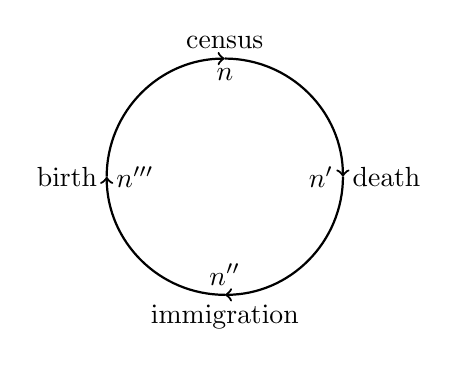
\begin{tikzpicture}[scale = 1.5]
				% circle and arrow heads
				\draw[->, thick] (-10mm, 0mm) arc (180:90:10mm);
				\draw[->, thick] (0mm, 10mm) arc (90:0:10mm);
				\draw[->, thick] (10mm, 0mm) arc (0:-90:10mm);
				\draw[->, thick] (0mm, -10mm) arc (-90:-180:10mm);
				
				% events
				\draw (0, 10mm) node[anchor=south] {census};
				\draw (10mm, 0mm) node[anchor=west] {death};
				\draw (0mm, -10mm) node[anchor=north] {immigration};
				\draw (-10mm, 0mm) node[anchor=east] {birth};
				
				% variables
				\draw (0, 10mm) node[anchor=north] {$n$};
				\draw (10mm, 0mm) node[anchor=east] {$n'$};
				\draw (0mm, -10mm) node[anchor=south] {$n''$};
				\draw (-10mm, 0mm) node[anchor=west] {$n'''$};
				
			\end{tikzpicture}
			\end{center}
			\caption{Life-cycle diagram for a squirrel model with alternative order of events.}
			\label{fig:lcdsquirrelsalt}
		\end{figure}
	\item[P.1.2] The flow diagram is shown in Fig.\ \ref{fig:fldismodel}. The parameter $\gamma$ is the rate at which infected individuals recover and become susceptible again. The parameter $\nu$ denotes an additional death rate experienced by infected individuals as compared to the death rate $d$ of susceptible ones.
		\begin{figure}[!bth]
			\begin{center}
			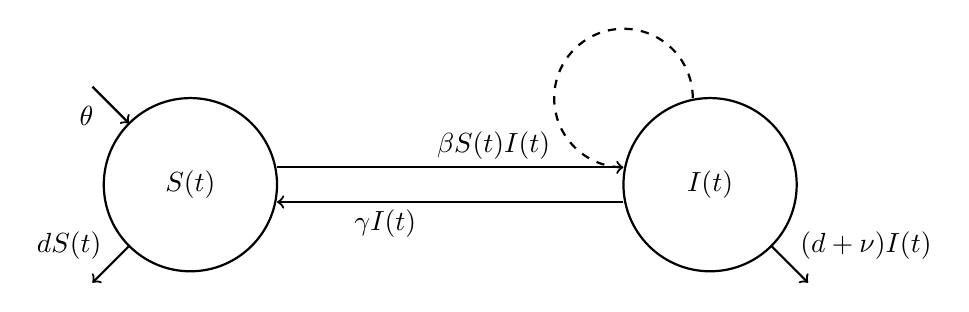
\begin{tikzpicture}[scale = 1.1]
				% circles
				\draw[thick] (-30mm, 0mm) circle (10mm);
				\draw[thick] (30mm, 0mm) circle (10mm);
				
				% arrows
				\draw[->, thick] (-20mm, 2mm) -- (20mm, 2mm);
				\draw[->, thick] (20mm, -2mm) -- (-20mm, -2mm);
				\draw[<-, thick] (-37.07107mm, 7.07107mm) -- (-41.3137mm, 11.3137mm);
				\draw[->, thick] (-37.07107mm, -7.07107mm) -- (-41.3137mm, -11.3137mm);
				\draw[->, thick] (37.07107mm, -7.07107mm) -- (41.3137mm,  -11.3137mm);
				\draw[thick, dashed] (28mm, 10mm) arc (0:270:8mm);
				
				% variables
				\draw (-30mm, 0mm) node {$S(t)$};
				\draw (30mm, 0mm) node {$I(t)$};
				
				% flows
				\draw (-42mm, 8mm) node {$\theta$};
				\draw (-44mm, -7mm) node {$d S(t)$};
				\draw (48mm, -7mm) node {$(d + \nu) I(t)$};
				\draw (-7.5mm, -4.5mm) node {$\gamma I(t)$};
				\draw (5mm, 4.5mm) node {$\beta S(t) I(t)$};
				
			\end{tikzpicture}
			\end{center}
			\caption{Flow diagram for the continuous-time model of Problem P.1.2.}
			\label{fig:fldismodel}
		\end{figure}
	\item[P.1.3] The flow diagram is as given in Fig.\ \ref{fig:lsdirsmodel}, and the continuous-time differential equations are
		\begin{subequations}
			\label{eq:lsdirsmodel}
			\begin{align}
				\frac{ds}{dt} &= \sigma r(t) - a c s(t) n(t)\\
				\frac{dn}{dt} &= a c s(t) n(t) - \rho n(t)\\
				\frac{dr}{dt} &= \rho n(t) - \sigma r(t)
			\end{align}
		\end{subequations}
		\begin{figure}[!bth]
			\begin{center}
			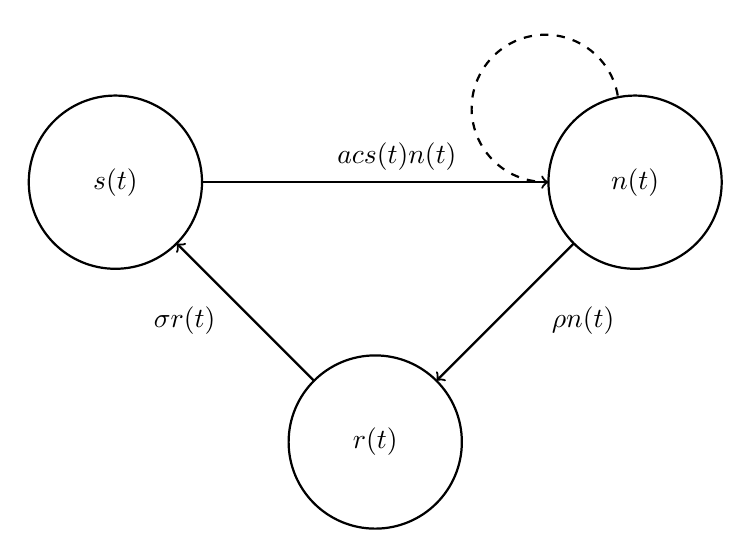
\begin{tikzpicture}[scale = 1.1]
				% circles
				\draw[thick] (-30mm, 0mm) circle (10mm);
				\draw[thick] (30mm, 0mm) circle (10mm);
				\draw[thick] (0mm, -30mm) circle (10mm);
				
				% arrows
				\draw[->, thick] (-20mm, 0mm) -- (20mm, 0mm);
				\draw[<-, thick] (-22.92803mm, -7.07107mm) -- (-7.07107mm, -22.92003mm);
				\draw[->, thick] (22.92803mm, -7.07107mm) -- (7.07107mm, -22.92003mm);
				\draw[thick, dashed] (28mm, 10mm) arc (10:270:8.5mm);
				
				% variables
				\draw (-30mm, 0mm) node {$s(t)$};
				\draw (30mm, 0mm) node {$n(t)$};
				\draw (0mm, -30mm) node {$r(t)$};
				
				% flows
				\draw (-22mm, -16mm) node {$\sigma r(t)$};
				\draw (24mm, -16mm) node {$\rho n(t)$};
				\draw (2.5mm, 3mm) node {$a c s(t) n(t)$};
				
			\end{tikzpicture}
			\end{center}
			\caption{Flow diagram for the continuous-time version of the flu model of Problem P.1.3, with an additional class of resistant individuals.}
			\label{fig:lsdirsmodel}
		\end{figure}
\end{enumerate}


\section{Chapter 2}

\begin{enumerate}
	\item[P.2.1] We start from the discrete-time difference equation for the exponential growth model,
		\begin{equation}
			\Delta n = n(t+1) - n(t) = R n(t) - n(t) = (R - 1) n(t)
		\end{equation}
		We recall that the reproductive factor was given by $R = (1+b)(1-d)$, where $b$ and $d$ are the number of offspring per adult female and the proportion of individuals dying per generation, respectively. Moreover, we recall that the growth rate was defined as $r_d = R - 1 = b - d - b d$. Therefore, the difference equation can be written as
		\begin{equation}
			\Delta n = (R - 1) n(t) = r_d n(t) = (b - d - b d) n(t).
		\end{equation}
		To derive the differential equation, consider a small amount of time $\Delta t$, such that the number of offspring per adult female and the proportion of individuals dying during this time are now $b \Delta t$ and $d \Delta t$, respectively. Hence, $n(t+\Delta t) - n(t) = \left[b \Delta t - d \Delta t - b d (\Delta t)^2  \right] n(t)$. Applying the definition of the differential, we find
		\begin{equation}
		\begin{split}
			\frac{dn}{dt} & = \lim_{\Delta t \rightarrow 0} \frac{n(t+\Delta t) - n(t)}{\Delta t}\\
			& =  \lim_{\Delta t \rightarrow 0} \frac{\left[b \Delta t - d \Delta t - b d (\Delta t)^2  \right] n(t)}{\Delta t} \\
			& =  \lim_{\Delta t \rightarrow 0} (b - d - b d \Delta t) n(t)\\
			& = (b - d) n(t).
		\end{split}
		\end{equation}
		This implies that the continuous-time growth rate is $r_c = b - d$. Comparing to $r_d = b - d - bd$, we see that the interaction term $b d$ is lost when we switch from discrete to continuous time. This is because, in the limit of a time step becoming small, no more than one type of event occurs. In continuous time, individuals that are born in a small amount of time will not suffer death in that same amount of time.
		
		\item[P.2.2] We start by recalling the continuous-time differential equation for the exponential growth model,
		\begin{equation}
			\label{eq:expgrowthcont}
			\frac{dn}{dt} = r_c n(t).
		\end{equation}
		To account for the effect of intra-specific competition for limited resources, we want $r_c$ to depend on population size as described in the problem. For this, the intercept needs to be equal to $r_c$ and the slope equal to $-r_c/K$. Hence,
		\begin{equation}
			r_c(n) = r_c + \left(-\frac{r_c}{K}\right) n(t) = r_c \left( 1 - \frac{n(t)}{K}\right).
		\end{equation}
		Substituting $r_c(n)$ for $r_c$ in Eq.\ \eqref{eq:expgrowthcont}, we obtain the solution
		\begin{equation}
			\frac{dn}{dt} = r_c \left( 1 - \frac{n(t)}{K}\right) n(t).
		\end{equation}
		
		\item[P2.3] Applying the quotient rule of differentiation, we find
		\begin{equation}
		\begin{split}
			\frac{dp}{dt} & = \frac{\frac{d n_A}{dt} \left(n_A + n_a \right) - n_A \left(\frac{d n_A}{dt} + \frac{d n_a}{dt} \right)}{\left(n_A + n_a \right)^2}\\
			& = \frac{n_a \frac{d n_A}{dt} - n_A \frac{d n_a}{dt}}{\left(n_A + n_a \right)^2}.
		\end{split}
		\end{equation}
		Substitution of $d n_A / dt = r_A n_A(t)$ and $d n_a / dt = r_a n_a(t)$ yields
		\begin{equation}
		\begin{split}
			\frac{dp}{dt} & = \frac{n_a (r_A n_A) - n_A (r_a n_a)}{\left(n_A + n_a \right)^2} \\
			& = (r_A - r_a) \frac{n_A n_a}{\left(n_A + n_a \right)^2} = (r_A - r_a) p(t) q(t),
		\end{split}
		\end{equation}
		using $q(t) = 1 - p(t) = n_a(t) / (n_A(t) + n_a(t))$. Note that in the derivation we have omitted the dependence of $n_A$ and $n_a$ on $t$ in our notation for simplicity. Comparing the result to the differential equation derived earlier, $dp / dt = s_c p(t) q(t)$, we see that the continuous-time selection coefficient $s_c$ can be interpreted as the difference between the intrinsic growth rates of the two haploid genotypes that compete.
\end{enumerate}